\chapter{Paralelización con sistemas homogéneos y heterogéneos}

Este capítulo explora las técnicas de paralelización en sistemas homogéneos y heterogéneos. Comienza con una revisión de los tipos de paralelismo, diferenciando el paralelismo del modelo y el paralelismo de datos, y describe cómo se aplican en las implementaciones del proyecto: OpenMP utiliza paralelismo de datos, mientras que CUDA y cuDNN se basan en paralelismo del modelo.

Luego, se detalla la paralelización en sistemas homogéneos mediante OpenMP, con un enfoque para la paralelización del descenso por gradiente estocástico (SGD).

El capítulo continúa con la paralelización en sistemas heterogéneos, que abarca desde las operaciones Producto Matriz-Matriz General (GEMM) y su aplicación en convoluciones y capas totalmente conectadas, hasta la memoria requerida para GEMM y la retropropagación en capas convolucionales. Finalmente, se analiza la multiplicación de matrices en CUDA y el flujo de ejecución en estos sistemas.


\section{Tipos de paralelismo}

El entrenamiento de una red neuronal convolucional (CNN) se puede paralelizar de diversas maneras. Cuando el modelo se divide entre varios ordenadores que son entrenados con los mismos datos, se conoce como \textbf{paralelismo del modelo} \cite{data_model_parallelism} (por ejemplo, asignando una capa por computador). Por otro lado, cuando se distribuyen los datos entre múltiples nodos, pero se utiliza el mismo modelo para el entrenamiento en cada uno de ellos, se denomina \textbf{paralelismo de datos} \cite{model_parallelism}. En este proyecto, la implementación con OpenMP se basará en un paralelismo de datos, mientras que las implementaciones heterogéneas, utilizando CUDA y cuDNN, aprovecharán el paralelismo del modelo. \\

\section{Paralelización en sistemas homogéneos mediante OpenMP}

\begin{algorithm}[H]
	\caption{Descenso del gradiente estocástico mediante OpenMP} 
	\begin{algorithmic}
		\State Datos de entrenamiento $D=\{(x_1, y_1), (x_2, y_2), ..., (x_N, y_N)\}$.
		
		\For{cada trabajador $t =0, ..., T-1$ en paralelo}
		\For{época $p\in\{0, ..., P-1\}$}
		\State Desordenar vector de datos D.
		\For{cada mini batch $m =0, ..., M-1$}
		\State Inicializar $gradientes^t$ a 0.
		\State Reparto de datos del batch m al trabajador t
		\State Realizar propagación hacia delante
		\State Obtener error total con la función de pérdida
		\State Cada trabajador t realiza la propagación hacia 
		\State detrás y obtiene el gradiente con respecto a 
		\State cada parámetro del modelo.
		
		\State Acumular gradientes obtenidos por cada trabajador t.
		\State Actualizar parámetros.
		
		\EndFor
		\EndFor
		\EndFor
	\end{algorithmic}
\end{algorithm}

La naturaleza iterativa del algoritmo del descenso del gradiente estocástico, podría parecer un impedimento para la paralelización del entrenamiento del modelo, ya que, la iteración \textit{i}, depende del resultado obtenido en la iteración \textit{i-1}. Sin embargo, tal y como se expone en \cite{CNN_parallel_Stanford}, \cite{CNN_parallel_International_Conference}, y \cite{CNN_parallel_Ome_Weird_Trick}, es posible implementar paralelismo en cada iteración del proceso. \\
En cada época el modelo, se entrena con \textit{M} subconjuntos de $N_m$ datos, los cuales son disjuntos entre sí. Dados \textit{T} ``trabajadores'' o procesos paralelos, cada subconjunto de $N_m$ datos (mini-batch), puede dividirse en \textit{T} subconjuntos de $\frac{N_m}{T}$ datos, asignando cada uno a un trabajador diferente.\\
De acuerdo con este enfoque, los datos de entrenamiento se distribuyen entre los distintos trabajadores \textit{T} tanto para la propagación hacia delante como para la retropropagación posterior. En el caso de la retropropagación, se debe acumular el gradiente de la pérdida con respecto a cada parámetro obtenido por cada trabajor. Una vez en posesión de este gradiente `total', se procede a la actualización de los parámetros del modelo.

\begin{figure}[H]
	\centering
	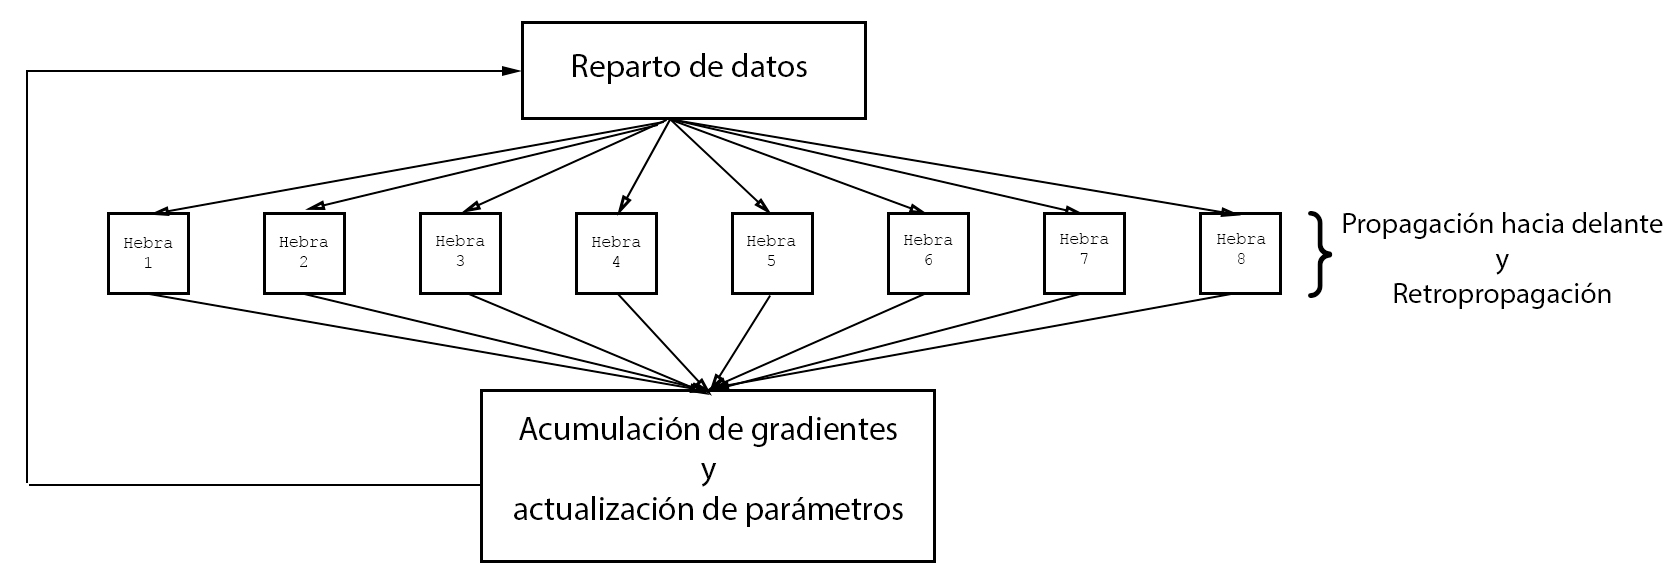
\includegraphics[width=1.2\linewidth]{imagenes/openmp_flujo.jpg} 
	\caption{Flujo de datos entre las hebras en la implementación con OpenMP}
	\label{fig:openmp_flujo}
\end{figure}

Tal como se muestra en la Figura \ref{fig:openmp_flujo}, aunque cada hebra realiza ciertas secciones de código en paralelo, como la propagación hacia delante o la retropropagación, existen momentos en los que estas hebras deben sincronizarse, como ocurre durante la distribución de los datos de un minibatch, o coordinarse para llevar a cabo operaciones conjuntas, como ocurre cuando se produce la acumulación y actualización de pesos.


\section{Paralelización en sistemas heterogéneos}
Una vez comprendidos los cálculos empleados por una CNN, en esta sección, se introducirá la metodología para llevar a cabo estos cálculos desde una perspectiva heterogénea. Es decir, mediante el uso de unidades de procesamiento gráfico (GPU) para la multiplicación matricial.

\subsection{GEMM}

El enfoque GEMM \cite{GEMM_definition} (General Matrix Multiply o Multiplicación General de Matrices), es ampliamente reconocido en el campo del aprendizaje profundo, y se utiliza en numerosas bibliotecas especializadas, como Caffe, Torch-cunn, Theano-CorrMM, o incluso CuDNN \cite{conv_GEMM_FFT_comparacion}. \\
En el contexto de redes neuronales convolucionales, el método GEMM facilita una reducción significativa en el tiempo de cómputo requerido. Sin embargo, esta optimización conlleva un incremento en el espacio de memoria necesario. 

\subsection{Convolución como GEMM \label{Intro_GEMMM}}

En el contexto de las capas convolucionales, la aplicación del enfoque GEMM (General Matrix Multiply), implica un proceso de ``desenrrollado'' tanto del volumen de entrada \textit{X}, como de la matriz de filtros \textit{K}. Este proceso, incluye la creación de una nueva matriz 2D, denominada $X_{unroll}$, donde, cada columna de dicha matriz, contiene todos los elementos de \textit{X} necesarios para calcular una posición específica del volumen de salida \textit{Y}. Dado que los resultados de cada convolución se suman a lo largo de cada canal de profundidad, estos pueden ser organizados en una matriz de gran tamaño. En este enfoque, cada kernel de pesos \textit{K}, se transforma en una fila de una extensa matriz de pesos denominada $M_{K}$. Este procedimiento, se ilustra en la Figura \ref{fig:conv_std_vs_gemm}, donde, los kernels \textit{K} y \textit{G}, se representan en colores verde y marrón, respectivamente. \\
Mientras que el método estándar, requiere varias iteraciones para calcular cada valor del volumen de salida \textit{Y}, (como se ilustra en la Figura \ref{fig:forward_prop_convolucional}), el enfoque GEMM, permite que cada valor de \textit{Y} se obtenga mediante la multiplicación de una fila de la matriz de pesos $M_{K}$, (ilustrada como verde y marrón en la Figura \ref{fig:conv_std_vs_gemm}), con una columna de la matriz $X_{unroll}$, (representada en azul en la Figura \ref{fig:conv_std_vs_gemm}). Esta técnica, detallada en \cite{Programming_Massively}, optimiza el tiempo de cómputo necesario para la operación de convolución, al transformar el problema en una multiplicación matricial que puede llevarse a cabo en GPU.
De este modo, dado un conjunto de \textit{M} filtros (kernels), de tamaño KxK, un volumen de entrada \textit{X} de dimensiones CxHxW, y un volumen de salida \textit{Y} de dimensiones $M \times H_{out} \times W_{out}$, la multiplicación matricial entre la matriz de pesos $M_{K}$, que posee M filas y $K^2 \times C$ columnas, y $X_{unroll}$ que contiene $K^2 \times C$ filas y $H_{out} \times W_{out}$ columnas, produce el mismo volumen de salida \textit{Y} que una convolución ordinaria con M kernels distintos. \\
Finalmente, aunque se haya omitido para simplificar la explicación del método, es necesario destacar que, una vez realizada la multiplicación matricial, se debe sumar el sesgo correspondiente, y aplicar la función de activación a cada elemento del volumen de salida \textit{Y}.

\begin{figure}[H]
	\hspace{-5mm}
	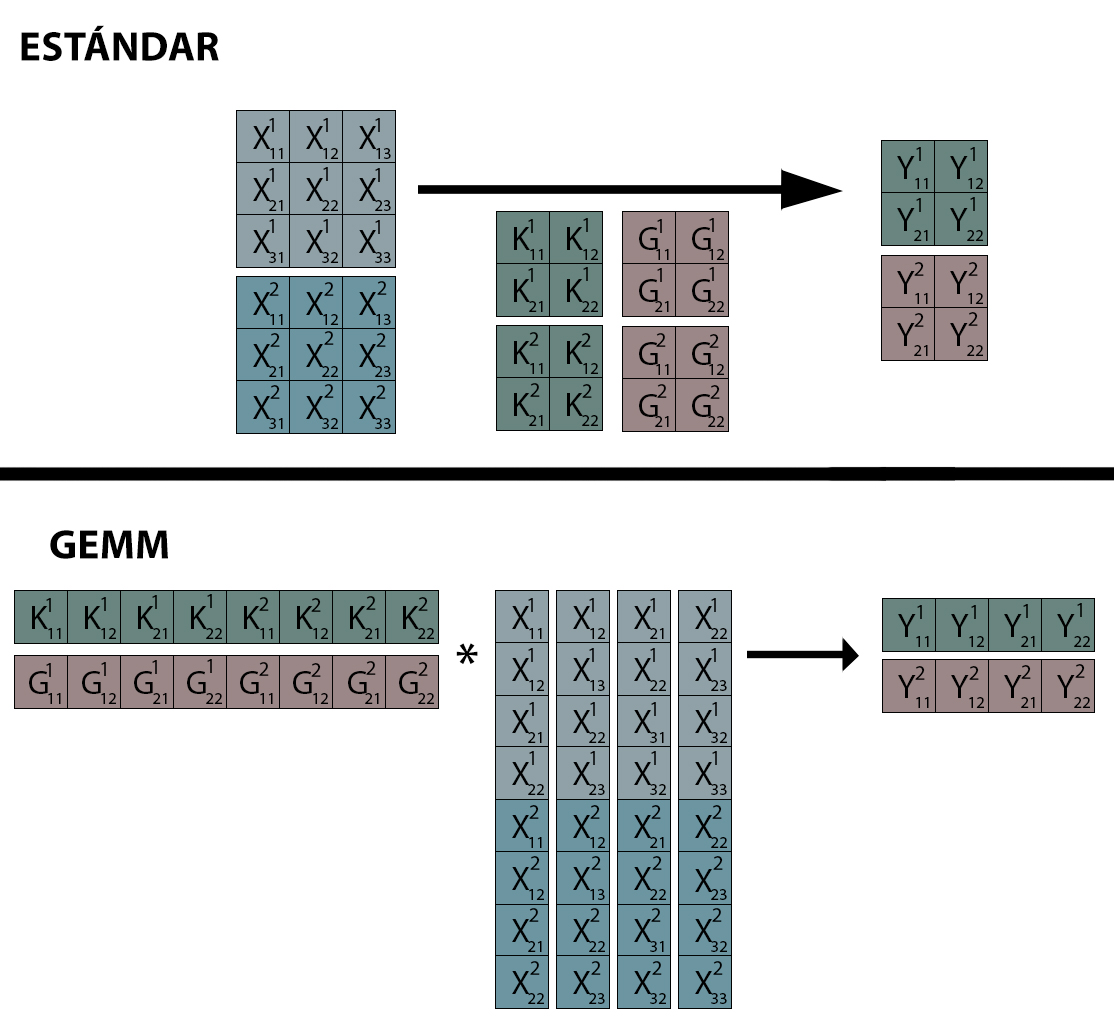
\includegraphics[scale=0.35]{imagenes/conv_std_vs_gemm.jpg}  
	\caption{Convolución estándar frente a convolución GEMM}
	\label{fig:conv_std_vs_gemm}
\end{figure}

\subsection{Memoria requerida al emplear GEMM}

Al realizar una convolución, un mismo filtro de pesos puede aplicarse a múltiples posiciones de la matriz de entrada \textit{X}. Esto, requiere duplicar los valores de la entrada \textit{X} en la matriz $X_{unroll}$, tantas veces como sea necesario para garantizar el acceso adecuado. Por ejemplo, en una matriz de entrada X de dimensiones (3$\times$3), y un kernel de pesos \textit{K} de (2$\times$2), (como se ilustra en la figura \ref{fig:conv_std_vs_gemm}), el valor central de X deberá duplicarse 4 veces, mientras que los valores en las posiciones laterales centrales se duplican dos veces, y los valores en las esquinas no requieren duplicación, ya que solo se accede a ellos una vez. De esta forma, una matriz inicial X de (3$\times$3) con 9 valores, se transforma en una matriz $X_{unroll}$ con 4$\times$1 + 2$\times$4 + 1$\times$4 = 16 valores, lo que genera un factor de expansión de 16/9 = 1.8 . \\
Cada valor de salida $Y^m_{ij}$, se obtiene a partir de la convolución de un kernel de K$\times$K pesos, aplicados a la entrada \textit{X}, a lo largo de sus \textit{C} canales de profundidad. Por lo tanto, el número de columnas de la matriz desenrrollada $X_{unroll}$, se define como C$\times$K$\times$K. De igual manera, dado que el resultado de la multiplicación de cada fila por cada columna de las matrices desenrolladas genera un valor $Y^m_{ij}$, la matriz $X_{unrolled}$ tiene tantas columnas como elementos en el volumen de salida \textit{Y}, es decir, $M \times H_{out} \times W_{out}$. \\
El ratio de expansión, se calcula mediante $\frac{C \times K \times K \times H_{out} \times W_{out}}{C \times H \times W}$, donde \textit{H} y \textit{W} representan las dimensiones de la entrada \textit{X} en términos de filas y columnas, respectivamente, y $H_{out}$ y $W_{out}$ corresponden a las filas y columnas de la salida \textit{Y}. En términos generales, cuando las dimensiones de la entrada \textit{X}, y, de la salida \textit{Y}, son considerablemente mayores que las del filtro de pesos \textit{K}, el ratio de expansión será de K$\times$K. \\
Cada kernel de pesos, con dimensiones K$\times$K, se representa como una fila dentro de la matriz total de pesos. Por lo tanto, la matriz total de pesos estará compuesta de K$\times$K filas, y \textit{M} columnas, siendo \textit{M} el número de filtros de pesos aplicados sobre la entrada \textit{X}. \\
Al realizar múltiples convoluciones sobre una misma entrada \textit{X}, (una por cada filtro de pesos distinto), es posible utilizar una única matriz expandida, denominada $X_{unrolled}$. Por otro lado, cuando se emplean filtros de pesos considerables, (como 5$\times$5 o mayores), la expansión de la matriz de entrada con un ratio de K$\times$K, puede generar matrices de tamaño excesivo. Dado que, el almacenamiento de todas las matrices de entrada expandidas, para un minibatch completo, podría resultar en un consumo de memoria significativo, se adopta una estrategia más eficiente. Esta consiste, en reservar un único espacio de memoria, con dimensiones $C \times K \times K \times H_{out} \times W_{out}$, (es decir, una instancia de $X_{unrolled}$), que se reutiliza para procesar cada dato del minibatch, optimizando así el uso de la memoria, y evitando la sobrecarga que supondría almacenar múltiples matrices expandidas simultáneamente \cite{Programming_Massively}.

\subsection{Retropropagación GEMM en capa convolucional}

En la figura \ref{fig:conv_backprop_como_convolucion_Y_K_pad}, se observó cómo la retropropagación, con respecto a la entrada en una capa convolucional, consiste en una convolución entre los kernels de pesos, y el volumen de salida. De manera análoga, en la Figura \ref{fig:conv_backprop_como_convolucion_Xpad_Y}, también se mostró cómo el gradiente con respecto a los pesos, se obtiene mediante una convolución entre el volumen de entrada, y el volumen de salida. \\
Dado que ambos gradientes se pueden implementar como convoluciones, y, considerando que en la sección \ref{Intro_GEMMM}, se demostró cómo implementar convoluciones utilizando el enfoque GEMM, es razonable asumir que la retropropagación en una capa convolucional, también se puede llevar a cabo mediante dicho enfoque.

\begin{figure}[H]
	\hspace{-40mm}
	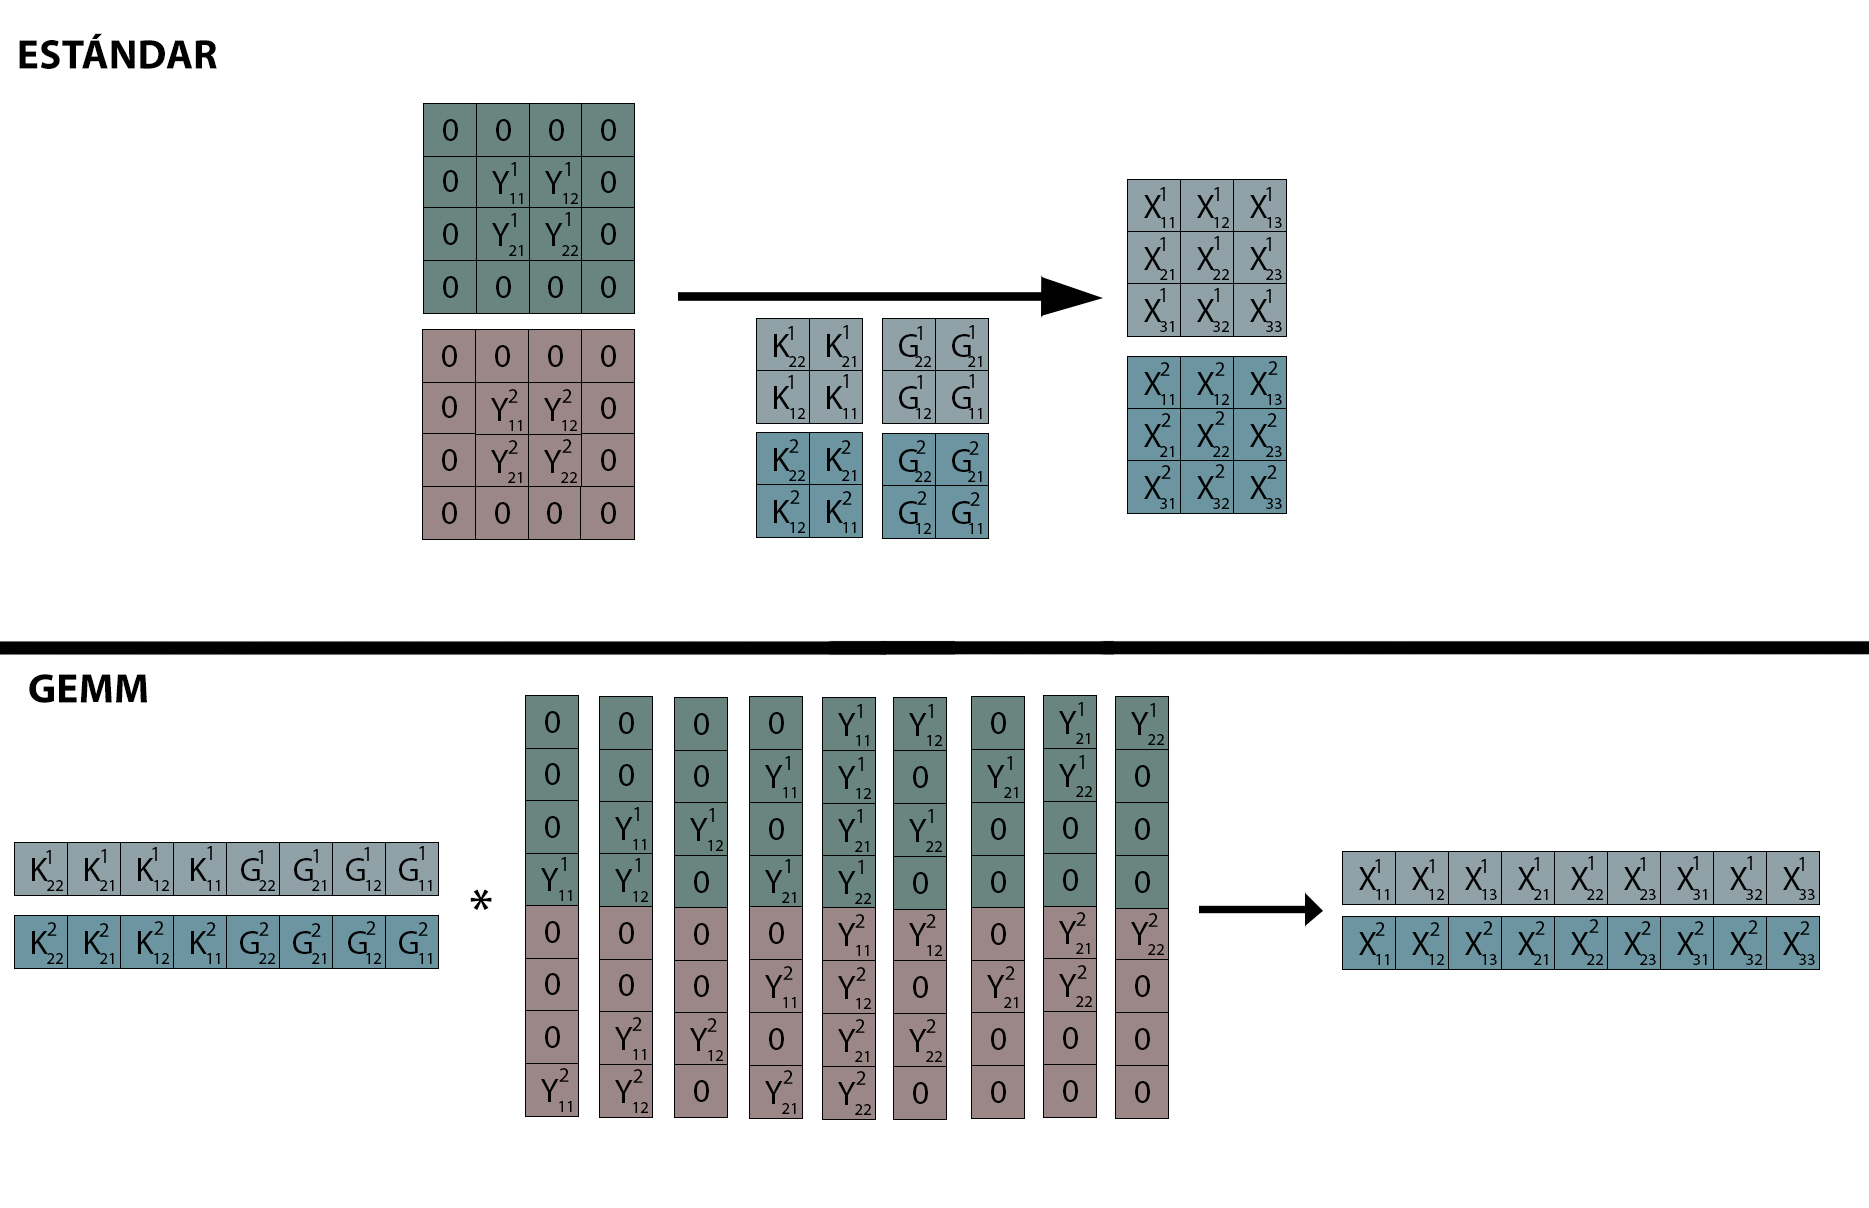
\includegraphics[scale=0.3]{imagenes/conv_std_vs_gemm_backprop.jpg}  
	\caption{Retropropagación respecto a la entrada en una capa convolucional de forma estándar frente a GEMM}
	\label{fig:conv_std_vs_gemm_backprop}
\end{figure}

En la Figura \ref{fig:conv_std_vs_gemm_backprop}, es importante destacar que, dado que canal de profundidad c$\in$C de cada kernel, solo influye en el correspondiente canal c del volumen de entrada \textit{X}, en la retropropagación, únicamente recibirá el gradiente proveniente de dicho canal. De esta manera, dado que cada kernel se utilizó para producir un canal m$\in$M distinto en el volumen de salida \textit{Y}, es posible concatenar los \textit{M} diferentes kernels para un mismo canal de profundidad c, de modo que, cada canal c, de cada kernel m, se multiplique por su subconjunto correspondiente en el canal m de \textit{Y}, e influya sobre el canal c de \textit{X}, (véase la Figura \ref{fig:conv_std_vs_gemm_backprop}). 

\begin{figure}[H]
	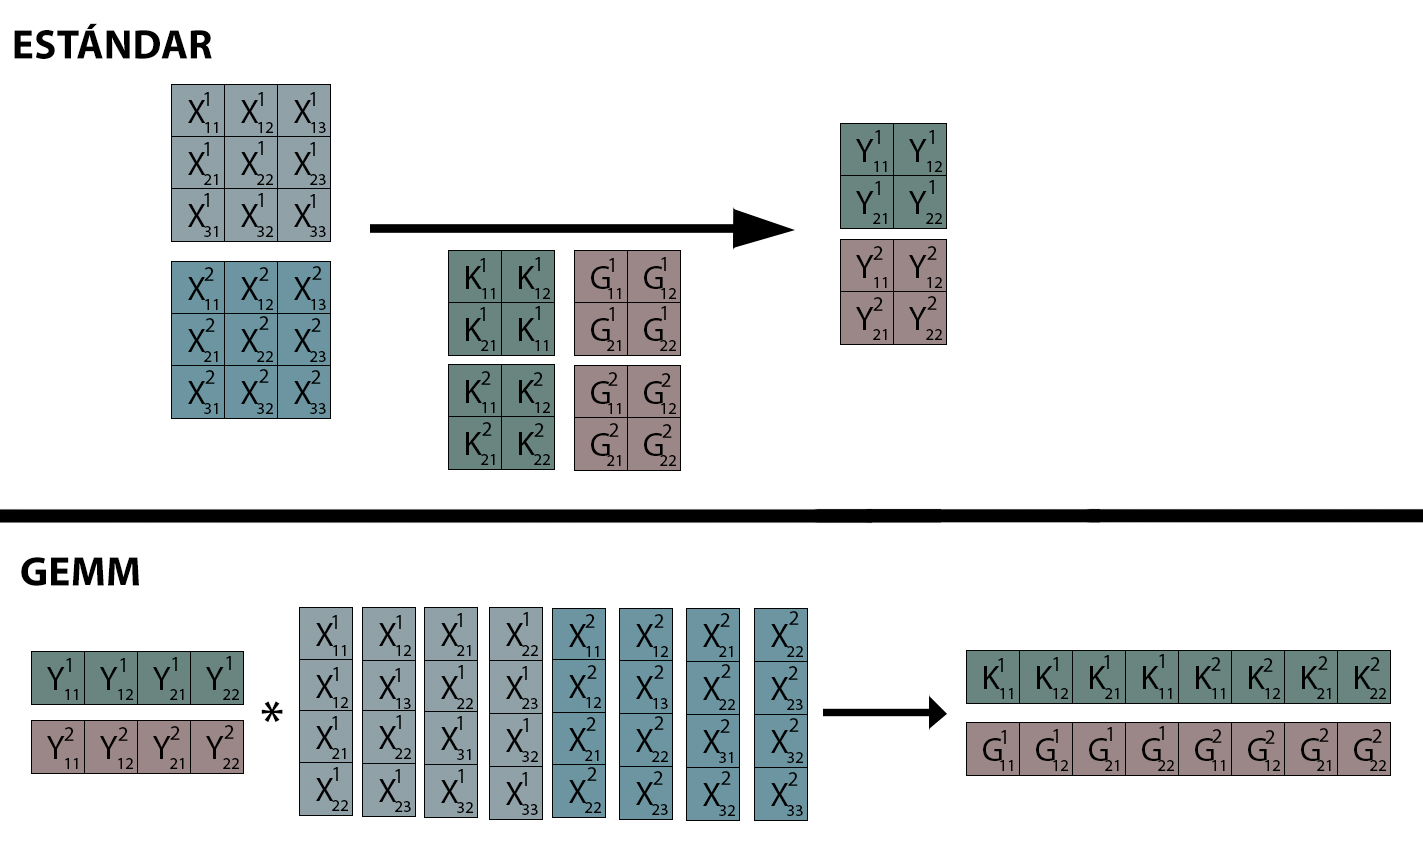
\includegraphics[scale=0.33]{imagenes/conv_std_vs_gemm_backprop_pesos.jpg}  
	\caption{Retropropagación respecto a los pesos en una capa convolucional de forma estándar frente a GEMM}
	\label{fig:conv_std_vs_gemm_backprop_pesos}
\end{figure}

En el caso del cálculo del gradiente de la pérdida con respecto a los pesos de una capa convolucional, cabe recordar que, este proceso, se puede implementar como una convolución entre el volumen de salida \textit{Y}, y el volumen de entrada \textit{X}. Utilizando el enfoque GEMM, tal como se ilustra en la Figura \ref{fig:conv_std_vs_gemm_backprop_pesos}, se observa que, para llevar a cabo esta operación, es necesario ``desenrrollar'' tanto el volumen de entrada X como el volumen de salida Y. De este modo, al multiplicar cada fila de Y (desenrrollado), por cada columna de X (desenrrollado), se multiplican todos los elementos del volumen de salida Y, y del volumen de entrada X, que, previamente, en la propagación hacia delante, fueron multiplicados por un peso distinto, calculando así el gradiente de dicho peso.

\subsection{Capa totalmente conectada como GEMM \cite{nvidia_back_fully_GEMM}}

Al igual que las capas convolucionales, las capas totalmente conectadas también se pueden implementar mediante un enfoque GEMM. Para ello, analizaremos por separado cada uno de los tres casos que se presentan:
\begin{enumerate}[label=\textbullet, nosep]
	\item Propagación hacia delante
	\item Cálculo del gradiente con respecto a la entrada
	\item Cálculo del gradiente con respecto a los pesos
\end{enumerate}

\subsubsection{Propagación hacia delante}

\begin{figure}[H]
	\centering
	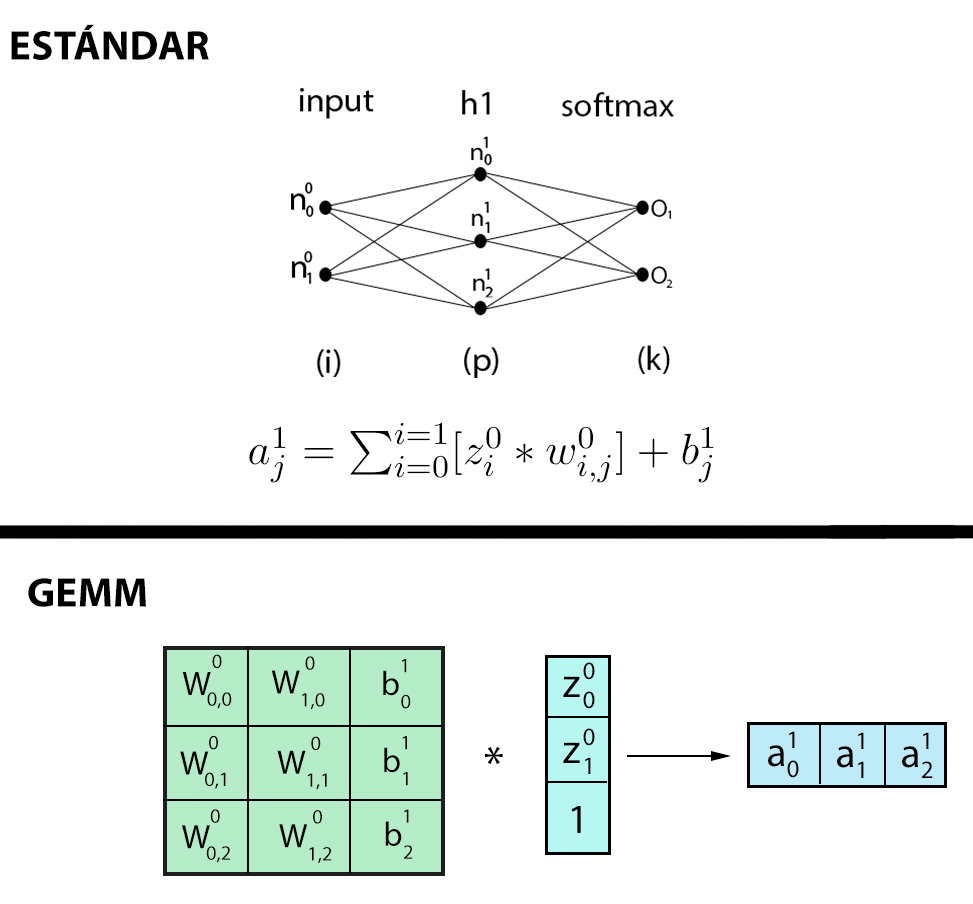
\includegraphics[scale=0.3]{imagenes/gemm_fully_forward.jpg}  
	\caption{Propagación GEMM hacia delante en una capa totalmente conectada}
	\label{fig:gemm_fully_forward}
\end{figure}

En la Figura \ref{fig:gemm_fully_forward}, se presentan dos enfoques distintos para implementar la propagación hacia delante en una capa totalmente conectada. El método \textbf{ESTÁNDAR}, se refiere al enfoque utilizado en secciones anteriores. En contraste, el método \textbf{GEMM}, ofrece una perspectiva alternativa para abordar esta tarea. Este enfoque implica, para una capa i, agrupar los pesos y sesgos de dicha capa en una matriz \texttt{M\_pesos\_sesgos}, y, por otro lado, utilizar una matriz \texttt{M\_neuronas} de una sola columna que contiene todas las neuronas de la capa i junto con un elemento adicional con valor igual a 1, que se emplea para sumar el sesgo. La matriz \texttt{M\_pesos\_sesgos} y la matriz \texttt{M\_neuronas} se ilustran en la Figura \ref{fig:gemm_fully_forward} mediante los colores verde y azul claro, respectivamente. \\
Siguiendo la estructura descrita en la Figura \ref{fig:gemm_fully_forward}, cada multiplicación de una fila de la matriz \texttt{M\_pesos\_sesgos} por una columna de la matriz \texttt{M\_neuronas} produce el valor de una neurona en la capa i+1. Para completar la propagación hacia delante de dicha capa, es necesario aplicar la función de activación a los resultados obtenidos.

\begin{figure}[H]
	\centering
	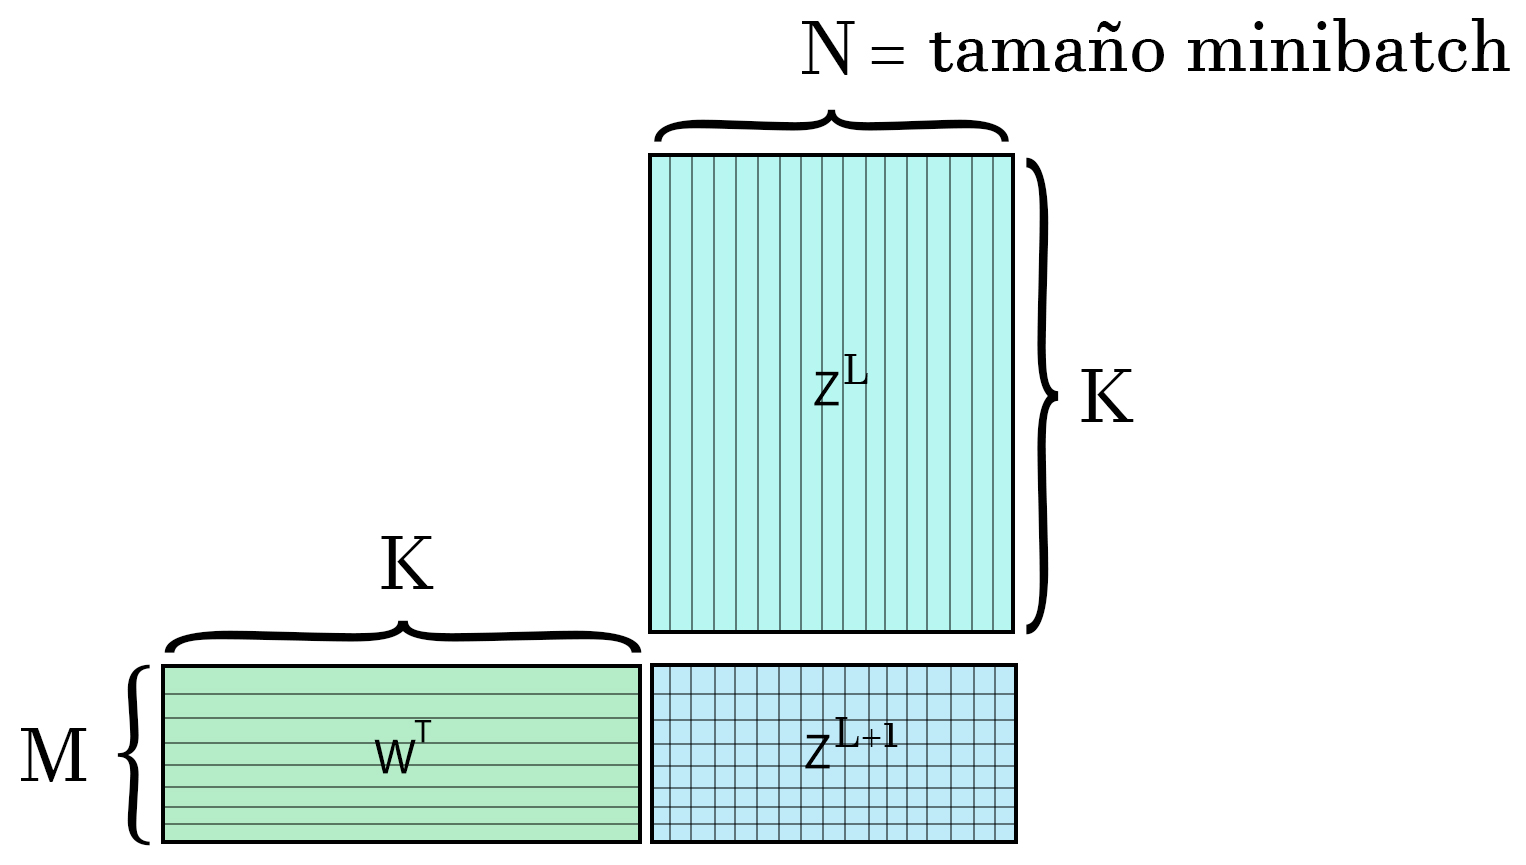
\includegraphics[scale=0.25]{imagenes/gemm_fully_forward_minibatch.jpg}  
	\caption{Propagación GEMM de un minibatch entero hacia delante en una capa totalmente conectada}
	\label{fig:gemm_fully_forward_minibatch}
\end{figure}

Dado que, los pesos y sesgos permanecen constantes durante todo un minibatch durante el entrenamiento, para un minibatch de tamaño \texttt{N}, podemos expandir la matriz \texttt{M\_neuronas} definida anteriormente para que tenga \texttt{N} columnas, una para cada elemento del minibatch. De esta manera, mediante una simple multiplicación matricial (enfoque GEMM), es posible realizar la propagación hacia delante de un minibatch completo para una capa totalmente conectada, tal como se muestra en la Figura \ref{fig:gemm_fully_forward_minibatch} \cite{nvidia_back_fully_GEMM}.

\newpage

\subsubsection{Retropropagación}

De manera similar a la propagación hacia delante, la retropropagación en una capa totalmente conectada también se puede calcular utilizando un enfoque de multiplicación matricial, como es el enfoque GEMM.

\subsubsection{Gradiente respecto a la entrada}
\begin{figure}[H]
	\centering
	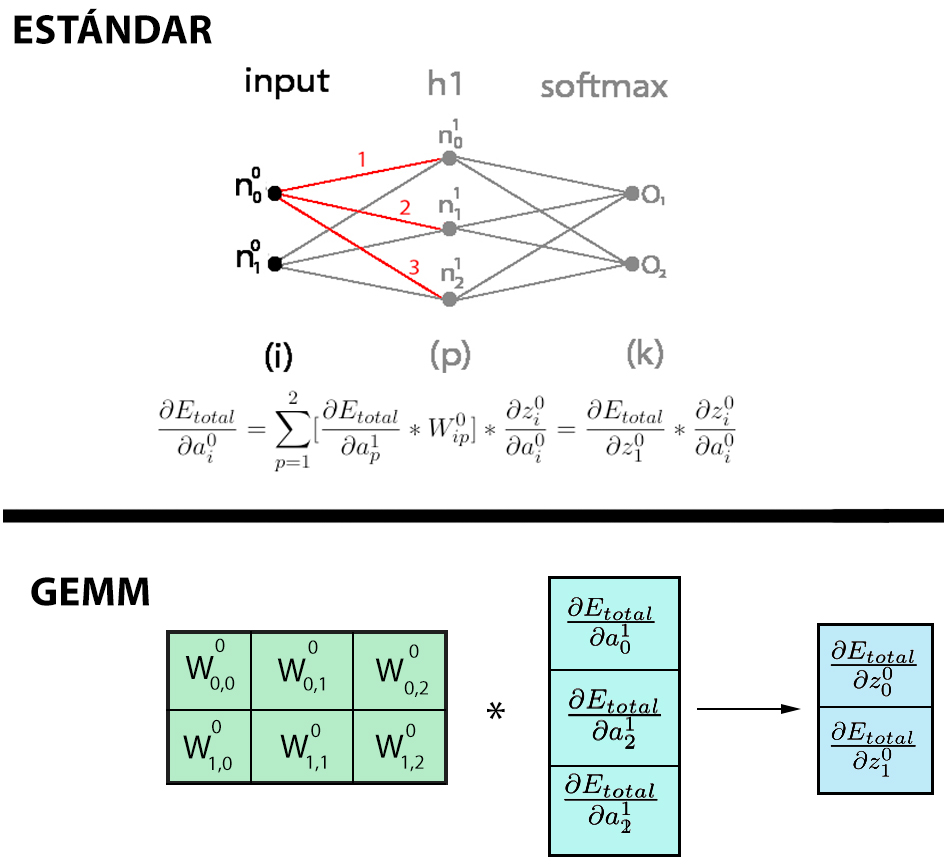
\includegraphics[scale=0.35]{imagenes/gemm_fully_back_input.jpg}  
	\caption{Cálculo del gradiente respecto a la entrada en una capa totalmente conectada}
	\label{fig:gemm_fully_back_input}
\end{figure}

Supongamos que estamos en la capa i, y ya disponemos del gradiente de la pérdida con respecto a la entrada de la capa i+1. En este caso, podemos calcular el gradiente con respecto a la entrada de la capa i, tal como se ilustra en la Figura \ref{fig:gemm_fully_back_input}. \\
En este contexto, se considera una matriz \texttt{pesos}, en la que cada fila j, contiene los pesos que conectan la neurona j de la capa i, con todas las neuronas de la capa i+1. La matriz \texttt{neuronas}, por su parte, tiene una sola columna y contiene las neuronas de la capa i+1. Sin embargo, en esta ocasión, las neuronas de esta matriz \texttt{neuronas} contienen el gradiente de la pérdida hasta esa capa. De este modo, cada multiplicación de una fila de \texttt{pesos}, por una columna de \texttt{neuronas}, produce el cálculo del gradiente de la pérdida con respecto a una neurona de entrada distinta. \\
En la Figura \ref{fig:gemm_fully_back_input}, se presenta tanto una representación visual de las matrices \texttt{neuronas}, y \texttt{pesos}, así como la fórmula utilizada en el método estándar. Esto, facilita una comprensión más clara, de que ambos métodos representan enfoques alternativos para lograr el mismo objetivo, produciendo así resultados equivalentes.

\begin{figure}[H]
	\centering
	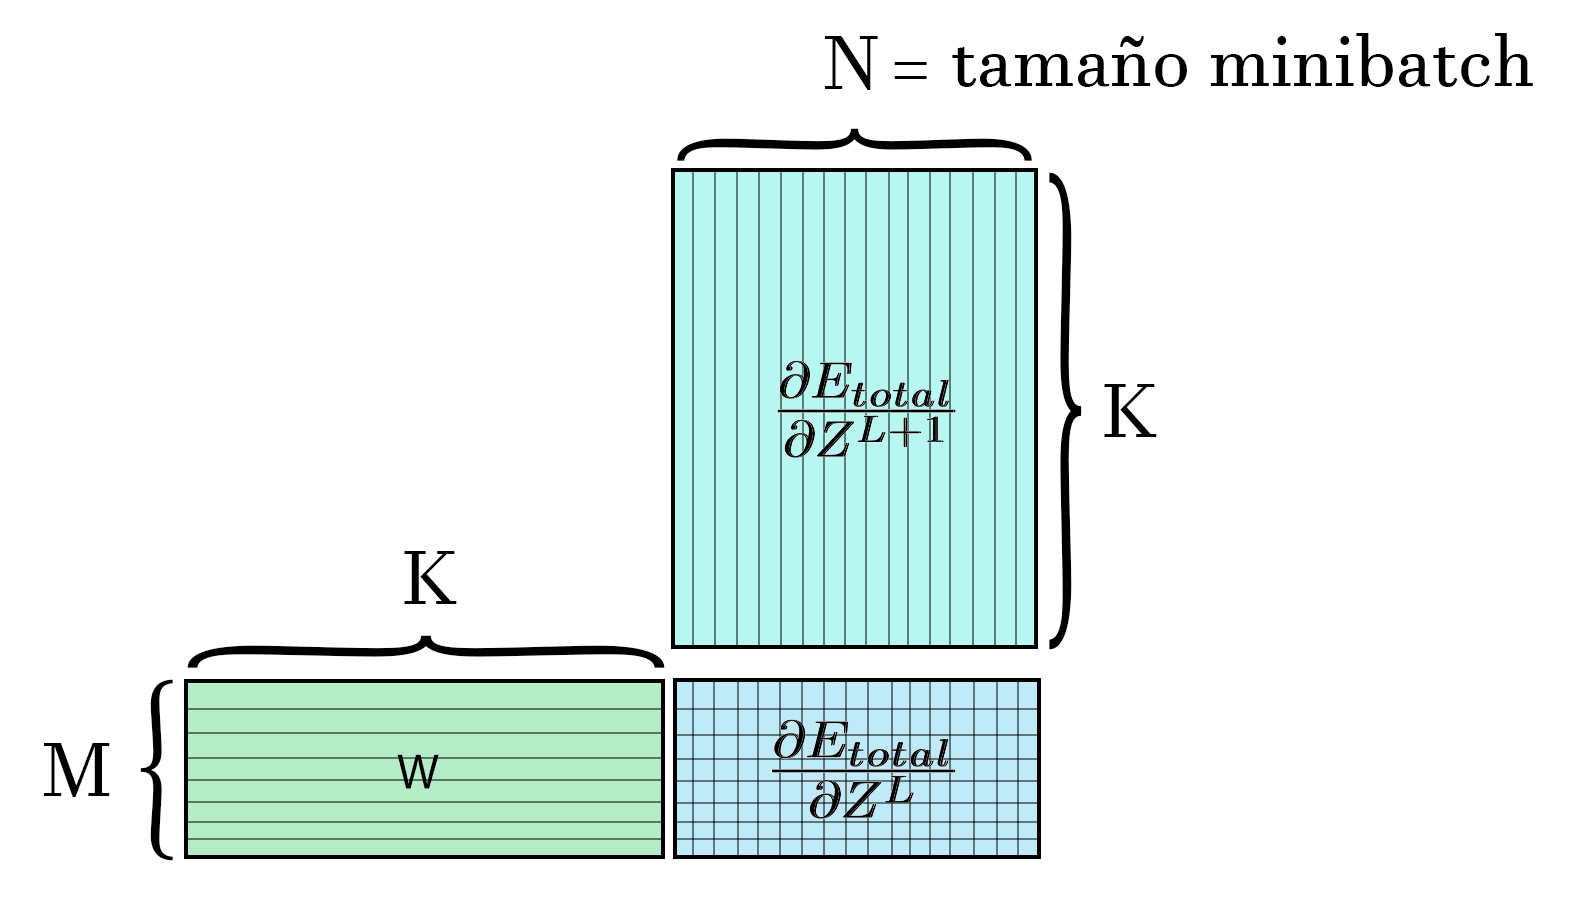
\includegraphics[scale=0.25]{imagenes/gemm_fully_back_input_minibatch.jpg}  
	\caption{Cálculo del gradiente respecto a la entrada de todo un minibatch en una capa totalmente conectada}
	\label{fig:gemm_fully_back_input_minibatch}
\end{figure}

De manera similar al apartado anterior, para un minibatch de \texttt{N} elementos, es posible expandir la matriz \texttt{neuronas} para que contenga \texttt{N} columnas. Esto, permite calcular el gradiente de la pérdida con respecto a la entrada para una capa i, a lo largo de todo el minibatch, mediante una simple multiplicación matricial, tal como se ilustra en la Figura \ref{fig:gemm_fully_back_input_minibatch}.

\subsubsection{Gradiente respecto a los pesos}
\begin{figure}[H]
	\centering
	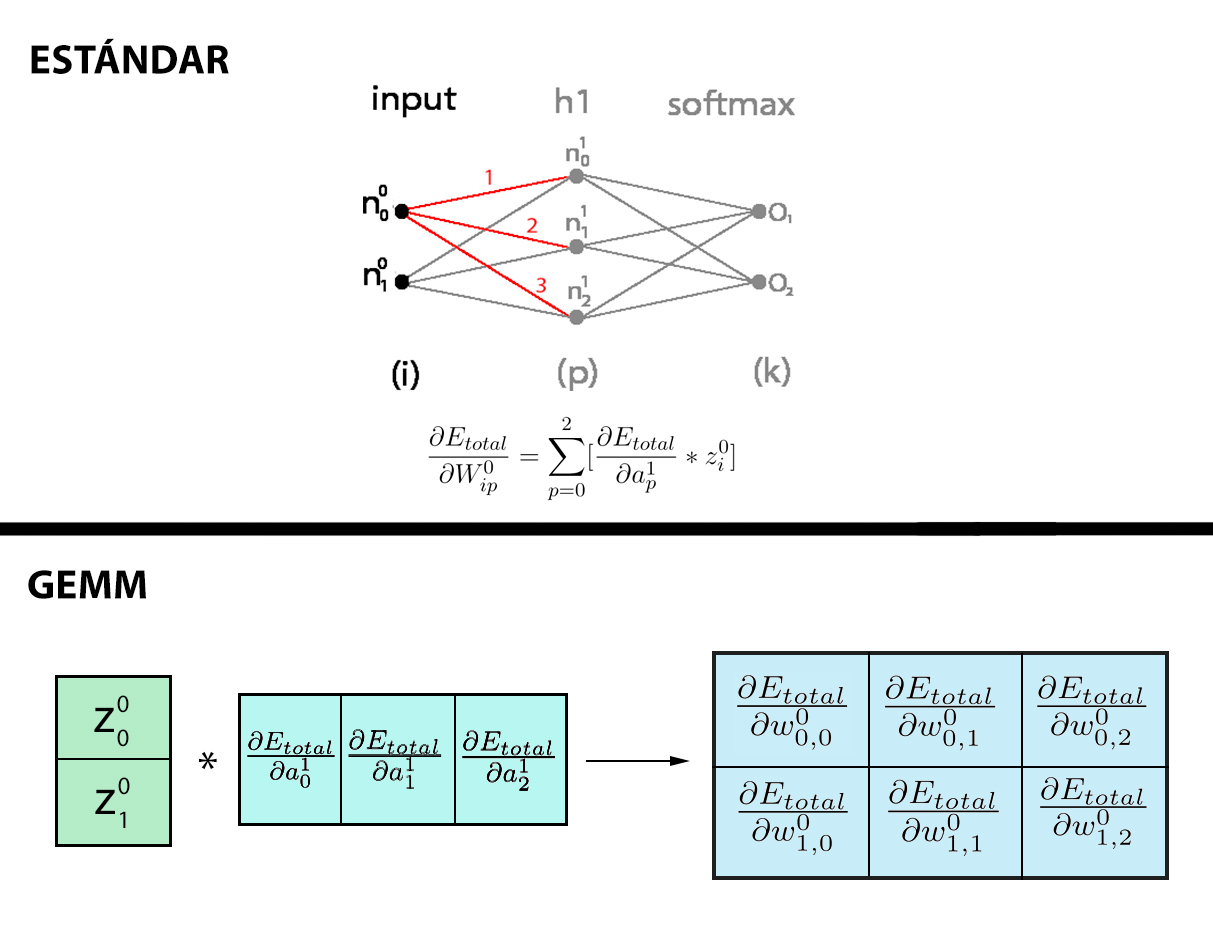
\includegraphics[scale=0.3]{imagenes/gemm_fully_back_w.jpg}  
	\caption{Cálculo del gradiente respecto a los pesos en una capa totalmente conectada}
	\label{fig:gemm_fully_back_w}
\end{figure}

En este caso, para una capa i, consideramos dos matrices que denominaremos \texttt{matriz\_entrada}, y \texttt{matriz\_salida}. La primera matriz, \texttt{matriz\_entrada}, se ilustra en color verde en la Figura \ref{fig:gemm_fully_back_w}, y se caracteriza por tener una sola columna que contiene las neuronas de entrada de la capa i. La segunda matriz, \texttt{matriz\_salida}, se muestra en color azul claro en la Figura \ref{fig:gemm_fully_back_w}, y tiene una sola fila, con el gradiente de la pérdida con respecto a cada neurona de salida de la capa i. De esta manera, cada multiplicación de una fila de \texttt{matriz\_entrada}, por una columna de \texttt{matriz\_salida}, produce el cálculo del gradiente de la pérdida con respecto a un peso que conecta una neurona de la capa i, con una neurona de la capa i+1. En otras palabras, se calcula el gradiente de la pérdida con respecto a los pesos de la capa i, tal y como se muestra en la Figura \ref{fig:gemm_fully_back_w}.

\begin{figure}[H]
	\centering
	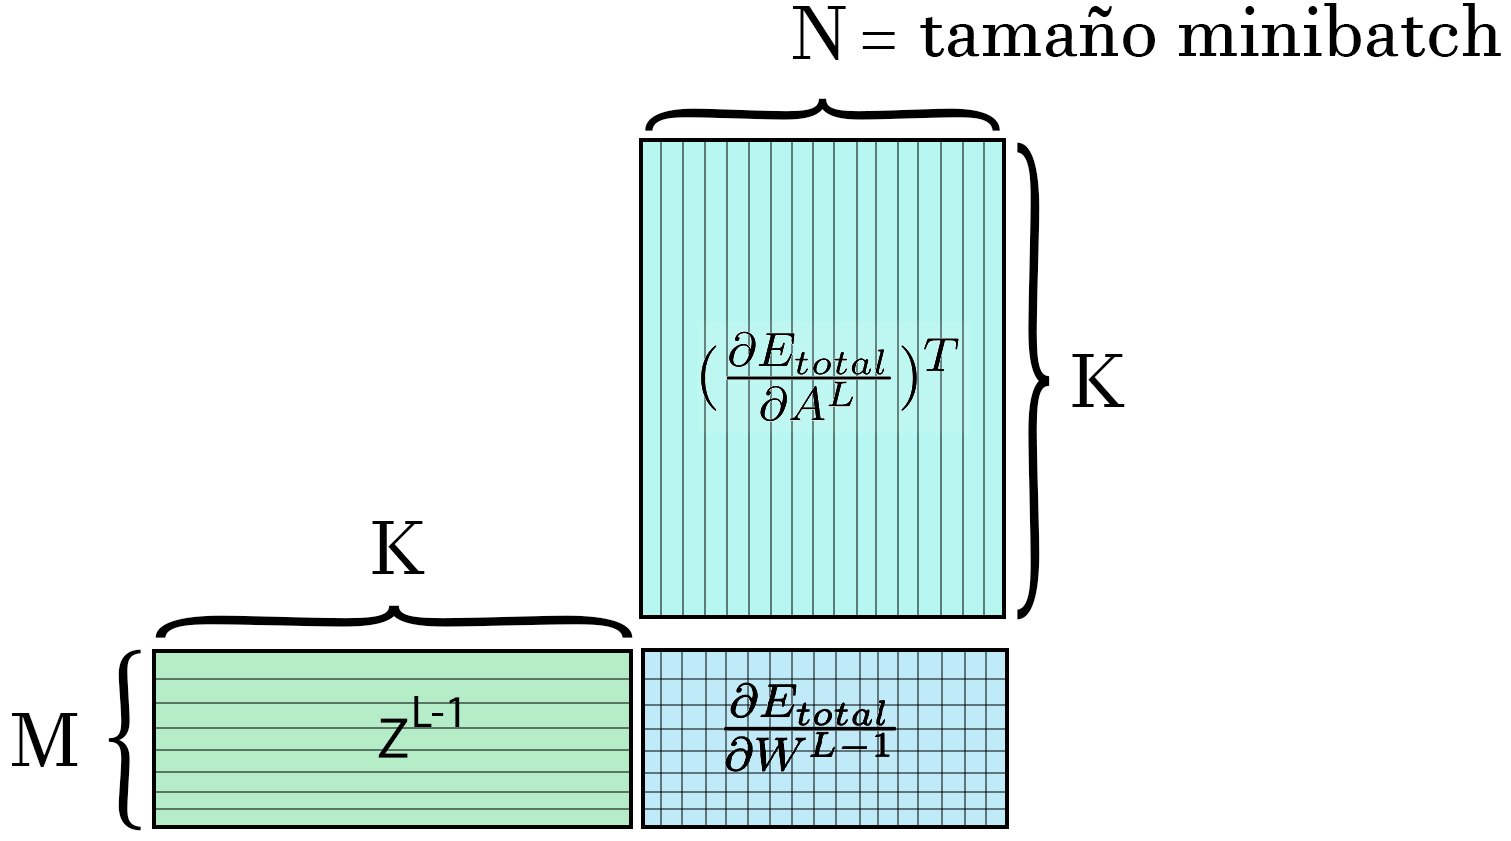
\includegraphics[scale=0.25]{imagenes/gemm_fully_back_w_minibatch.jpg}  
	\caption{Cálculo del gradiente respecto a los pesos de todo un minibatch en una capa totalmente conectada}
	\label{fig:gemm_fully_back_w_minibatch}
\end{figure}

Para un minibatch de tamaño \texttt{N}, se pueden expandir ambas matrices, de manera que cada una contenga \texttt{N} filas o columnas, según se indica en la Figura \ref{fig:gemm_fully_back_w_minibatch}. Esto, permite calcular el gradiente de la pérdida con respecto a los pesos para una capa i, en todo un minibatch, mediante una multiplicación matricial.

\subsection{Multiplicación de matrices en CUDA}

Dadas dos matrices \texttt{A} de tamaño M$\times$K, y \texttt{B} de tamaño K$\times$N, el producto de la multiplicación \texttt{AB} produce una matriz \texttt{C} de tamaño M$\times$N. Basándome en mi experiencia, una primera aproximación para realizar esta operación en CUDA, consiste en crear un bloque de tamaño K$\times$N, de manera que, cada hebra, calcule una posición de la matriz resultado \texttt{C}. Dada la simplicidad extrema de esta implementación, el desarrollador que la llevó a cabo, buscará formas de reducir el tiempo de cómputo requerido, optando en la mayoría de los casos por emplear memoria compartida de bloque. Tras desarrollar esta ``segunda versión'', el siguiente paso es comparar ambas implementaciones para verificar si realmente se obtiene una mejora significativa en el redimiento. \\
En el proceso, se observa que, para matrices de tamaño reducido, ambas implementaciones parecen funcionar adecuadamente. Sin embargo, a medida que aumenta el tamaño de las matrices, se detecta un claro ``tope'', debido a un defecto compartido por ambas: el tamaño de bloque. Por ejemplo, para calcular \texttt{C}(50$\times$50) = \texttt{A}(50$\times$10) x \texttt{B}(10$\times$50), ambas implementaciones requerirían un bloque de 50$\times$50 = 2500 hebras, lo cual excede el límite permitido por CUDA (1024 hebras por bloque). \\

\begin{figure}[H]
	\centering
	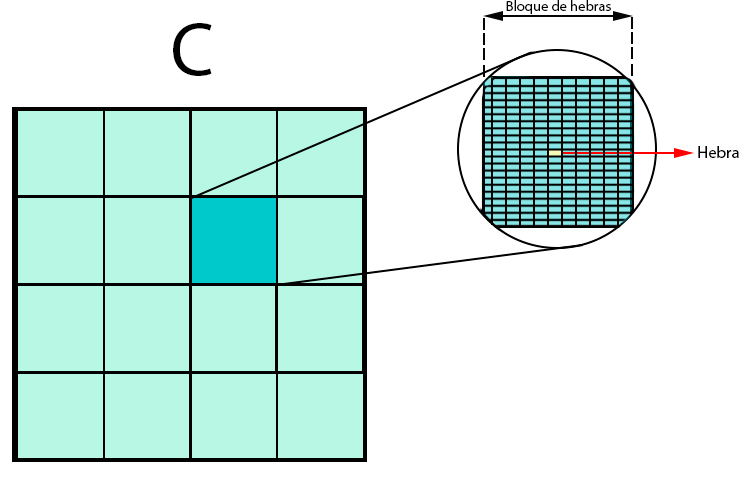
\includegraphics[scale=0.3]{imagenes/gemm_tile_v3.jpg}  
	\caption{Tercera implementación de multiplicación matricial con CUDA}
	\label{fig:mult_matrix_cuda_v3}
\end{figure}

Por lo tanto, resulta evidente la necesidad de una ``tercera'' implementación que carezca de este importante defecto. Esta, se caracteriza por dividir la matriz \texttt{C} en submatrices o \texttt{tiles}, de manera que, cada tile, corresponda a un bloque CUDA. A partir de las implementaciones anteriores, el cambio es inmediato, y los resultados son extraordinarios, ya que, esta solución, permite multiplicación matricial sin limitaciones de tamaño para \texttt{A} y \texttt{B}, además de ofrecer mejoras significativas en el rendimiento \cite{cuda_mult_matrix_v3}. \\
Sin embargo, esta última implementación carece de los beneficios que ofrece la memoria compartida a nivel de bloque, lo que sugiere, una vez más, la posible existencia de una mejora adicional sobre la misma. \\

\begin{figure}[H]
	\centering
	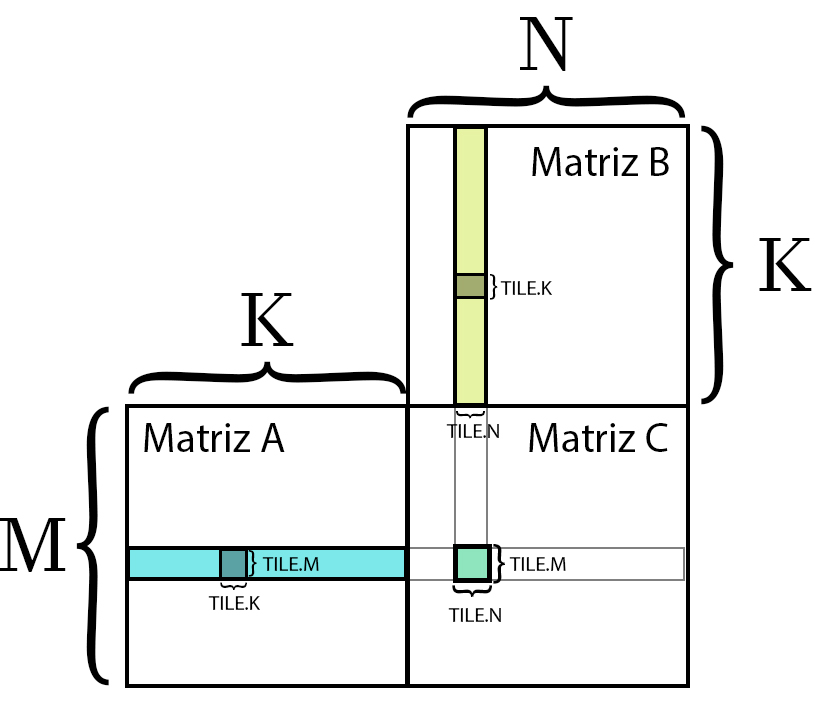
\includegraphics[scale=0.3]{imagenes/gemm_tile_v4.jpg}  
	\caption{Cuarta implementación de multiplicación matricial con CUDA}
	\label{fig:mult_matrix_cuda_v4}
\end{figure}

Para calcular cada valor de la matriz resultado \texttt{C}, es necesario multiplicar una fila de \texttt{A}, por una columna de \texttt{B}. Es decir, multiplicar dos vectores de \texttt{K} elementos. Una idea inicial, consiste en cargar \texttt{2K} elementos en memoria compartida para su posterior uso. Sin embargo, si cada hebra de cada bloque, requiere \texttt{2K} elementos, esta estrategia no es viable, debido a la limitada y escasa memoria compartida disponible. Un enfoque más eficiente consiste en, dado un bloque 2D de dimensiones \texttt{TILExTILE}, almacenar \texttt{2xTILExTILE} elementos, siendo \texttt{TILE} el tamaño de cada tile. El objetivo, es dividir el cálculo de cada valor de la matriz resultado \texttt{C}, en iteraciones, y, en cada una de ellas, cada hebra multiplica TILE elementos de \texttt{A}, por \texttt{TILE} elementos de \texttt{B}, acumulando y sumando los resultados obtenidos en cada iteración. De este modo, este será el método utilizado en el presente proyecto para realizar multiplicaciones matriciales en entornos heterogéneos, siguiendo las recomendaciones de NVIDIA en \cite{nvidia_mult_matrix_v4}. \\


\subsection{Flujo de ejecución}

\begin{figure}[H]
	\centering
	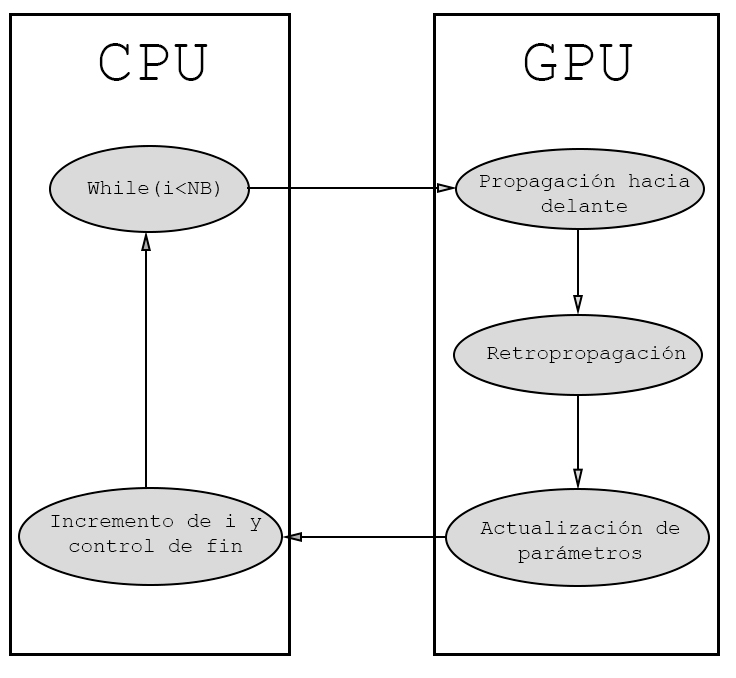
\includegraphics[width=0.8\linewidth]{imagenes/esquema_cpu_gpu.jpg} 
	\caption{Flujo de las hebras en la implementación con CUDA}
	\label{fig:cpu_gpu}
\end{figure}

Para llevar a cabo el entrenamiento en las implementaciones heterogéneas, los datos se cargan en la memoria de la GPU una única vez antes de iniciar el proceso, asegurando que todos los datos necesarios para el entrenamiento permanezcan en la GPU en todo momento, en lugar de en la CPU. Dado que el método de almacenamiento de datos empleado es idéntico tanto para la CPU como para la GPU (NCHW), este enfoque optimiza y simplifica el proceso. Una vez allí, la Figura \ref{fig:cpu_gpu} ilustra el flujo de ejecución para cada época de entrenamiento en la implementación con CUDA. Tal como se mencionó anteriormente, cada época se divide en \texttt{NB} minibatches. Durante cada uno de estos minibatches, la CPU se encarga de gestionar el inicio y la finalización, mientras que la GPU se ocupa del cómputo intensivo, que abarca la propagación hacia adelante, y la retropropagación, además de llevar a cabo la actualización de los parámetros.

De este modo, la CPU controla la mayor parte del flujo de control del programa. Por ejemplo, cuando es necesario realizar la propagación hacia delante o la retropropagación, la CPU invoca un kernel CUDA que se ejecuta en GPU, delegando a esta última todo el cómputo intensivo, como en el caso de la multiplicación matricial. Una vez finalizado dicho cómputo, el control regresa a la CPU, que se encarga de gestionar la invocación del siguiente kernel CUDA, así como de iniciar o finalizar cada minibatch. De esta manera, la implementación con cuDNN es muy similar a la implementación con CUDA. Sin embargo, en la implementación con CUDA, la CPU invoca kernels que se ejecutan en la GPU, mientras que en la implementación con cuDNN, la CPU llama a funciones de cuDNN, las cuales se encargan de todo el cómputo intensivo.
